\section{Исследовательская часть}

В данном разделе представлены описания исследований, проведенных для: оценки производительности программного обеспечения в зависимости от глубины рекурсии и от количества используемых дополнительных потоков при построении изображения, оценки реалистичности преломления света для прозрачных объектов в зависимости от входные параметров для материалов объектов; и сравнительный анализ результатов, полученных в ходе исследований.

\subsection{Технические характеристики}

Исследования проводилось на устройстве со следующими техническими характеристиками:

\begin{itemize}[label=---]
	\item операционная система macOS 14.6.1~\cite{macos};
	
	\item оперативная память (RAM) 16 ГБ;
	
	\item процессор (CPU) 2 ГГц 4‑ядерный Intel Core i5 (8 логических ядер)~\cite{intel}.
	
\end{itemize}

Во время проведения исследования, устройство было подключено к сети электропитания и не было нагружено сторонними приложениями, за исключением встроенных приложений окружения.

\subsection{Время построения изображения}

Далее будет приведен сравнительный анализ для исследований производительности программного обеспечения в зависимости от глубины рекурсии и от количества используемых дополнительных потоков при построении изображения.

Для замеров процессорного и реального времени выполнения построения изображения используются функция \textbf{std::clock\_t clock()} из библиотеки \textbf{<ctime>} и класс \textbf{std::chrono::high\_resolution\_clock} из библиотеки \textbf{<chrono>}, соответственно~\cite{ISO14882_2020}. Разница между начальным и конечным временем использовалась для получения точных результатов в секундах. Для входных данных измерения времени выполнения проводились по 10 раз. 

\subsubsection*{Влияние глубины рекурсии}

В реализации алгоритма обратной трассировки лучей задается глубина рекурсии, которая влияет на время построения изображения, а также на реалистичность изображения прозрачных объектов. В иследование производились замеры процессорного времени.

В таблице~\ref{rec-d} приведены результаты исследования времени построения изображения от глубины рекурсии. На рисунке~\ref{grp:dr} изображено графическое представление данных из таблицы~\ref{rec-d}.

\setcounter{table}{3}
\begin{table}[ht!]
	\begin{center}
		\caption{Время построения изображения}
		\begin{tabular}{ ||p{4cm}|r||  }
			\hline
			\multirow{1}{*}{Глубина рекурсии}& \multicolumn{1}{c||}{Время выполнения (с)} \\[1.5ex]
			\hline\hline
			0 & 2.709822 \\
			1  & 3.369566 \\
			2 &  3.967754 \\
			3 & 4.955640 \\
			4 & 7.129620 \\
			5 & 8.539870 \\
			6  & 11.750470 \\
			7 & 16.894780 \\
			8 & 24.755420 \\
			\hline
		\end{tabular}
		\label{rec-d}
	\end{center}
\end{table}

\begin{figure}[ht!]
	\begin{center}
		\begin{tikzpicture}
			\begin{axis}[
				legend pos = north west,
				xlabel=глубина~рекурсии,
				ylabel=секунды,
				grid = major,
				major grid style = {lightgray},
				minor grid style = {lightgray!25},
				xtick distance = 1,
				xmin=-0.2, 
				xmax= 8.2, 
				width = 1.0\textwidth,
				height = 0.45\textwidth,
				scaled y ticks=base 10:0,
				]
				
				\addplot[
				purple,
				semithick,
				mark = o,
				] file {./diag/dr.txt};
			\end{axis}
		\end{tikzpicture}
	\end{center}
	\caption{Зависимость времени построения изображения от глубины рекурсии}
	\label{grp:dr}
\end{figure}

\subsubsection*{Влияние использования дополнительных потоков}

В реализации алгоритма построения изображения используются дополнительные потоки, чтобы ускорить процесс вычисления цвета всех пикселей изображения, следовательно, использование дополнительных потоков влияет на реальное время построения изображения.

В таблице~\ref{th} приведены результаты исследования времени построения изображения от количества используемых дополнительных потоков. На рисунке~\ref{gth} изображено графическое представление данных из таблицы~\ref{th}. Замеры времени проводились при глубине рекурсии равной 4.

\begin{table}[ht!]
	\begin{center}
		\caption{Время построения изображения}
		\begin{tabular}{ ||p{4.5cm}|r||  }
			\hline
			\multirow{1}{*}{Количество потоков}& \multicolumn{1}{c||}{Время выполнения (с)} \\[1.5ex]
			\hline\hline
			1 & 	  5.10565 \\
			4  &     2.27339\\
			8 &  	 1.98203 \\
			16 &    1.73251 \\
			32 &    1.19489 \\
			64 &    1.08422 \\
			128 &   1.08445 \\
			256 &  1.09310 \\
			512 &   1.19786 \\
			1024 & 1.21875 \\
			\hline
		\end{tabular}
		\label{th}
	\end{center}
\end{table}

\begin{figure}[ht!]
	\begin{center}
		\begin{tikzpicture}
			\begin{axis}[
				legend pos = north west,
				xlabel=количество~потоков,
				ylabel=секунды,
				grid = major,
				major grid style = {lightgray},
				minor grid style = {lightgray!25},
				xtick={1,4,8,16,32,64,128,256,512,1024},
				xticklabels={1,~,~,~,~,64,~,~,512,1024},
				xmin=-10.0, 
				xmax= 1035, 
				width = 1.0\textwidth,
				height = 0.36\textwidth,
				scaled y ticks=base 10:0,
				]
				
				\addplot[
				purple,
				semithick,
				mark = o,
				] file {./diag/th.txt};
			\end{axis}
		\end{tikzpicture}
	\end{center}
	\caption{Зависимость времени построения изображения от количества используемых потоков}
	\label{gth}
\end{figure}

\subsection{Реалистичность преломления лучей}

Целью данного исследования является оценка влияния изменения коэффициента преломления на визуализацию прозрачных объектов в сцене.

Изменяя коэффициент преломления для жидкости или стекла, можно наблюдать, как меняется угол преломления лучей и, соответственно, видимость объектов через эти материалы. Следовательно, было исследованно, как различные значения коэффициентов преломления для стекла и жидкости влияют на искажения изображения объектов в сцене.

Были рассмотрены несколько комбинаций коэффициентов преломления для стекла и жидкости, которые описаны в таблице~\ref{comb}.

\begin{table}[ht!]
	\begin{center}
		\caption{Комбинации коэффициентов преломления для стекла и жидкости}
		\begin{tabular}{ ||p{3cm}||r|r||  }
			\hline
			\multirow{2}{*}{Номер}& \multicolumn{2}{c||}{Коэффициент преломления} \\[1.5ex]
			\cline{2-3} 
			комбинации& ~~~~~~~Стекло & Жидкость \\ [1.5ex] 
			\hline\hline
			1 & 1.0 & 1.0 \\
			2 & 1.0 & 1.5 \\
			3 & 1.3 & 1.0 \\
			4 & 1.3 & 1.5 \\
			\hline
		\end{tabular}
		\label{comb}
	\end{center}
\end{table}

На рисунке~\ref{c1} представлено изображение, полученное для комбинации №1 -- входных данных, где коэффициенты преломления для стекла и для жидкости равны 1. Изображение имеет наименьшее искажение света, что соответствует общепринятому поведению для одинаковых материалов.

\begin{figure}[ht!]
	\begin{center}
		\begin{minipage}{0.45\textwidth}
			\centering
			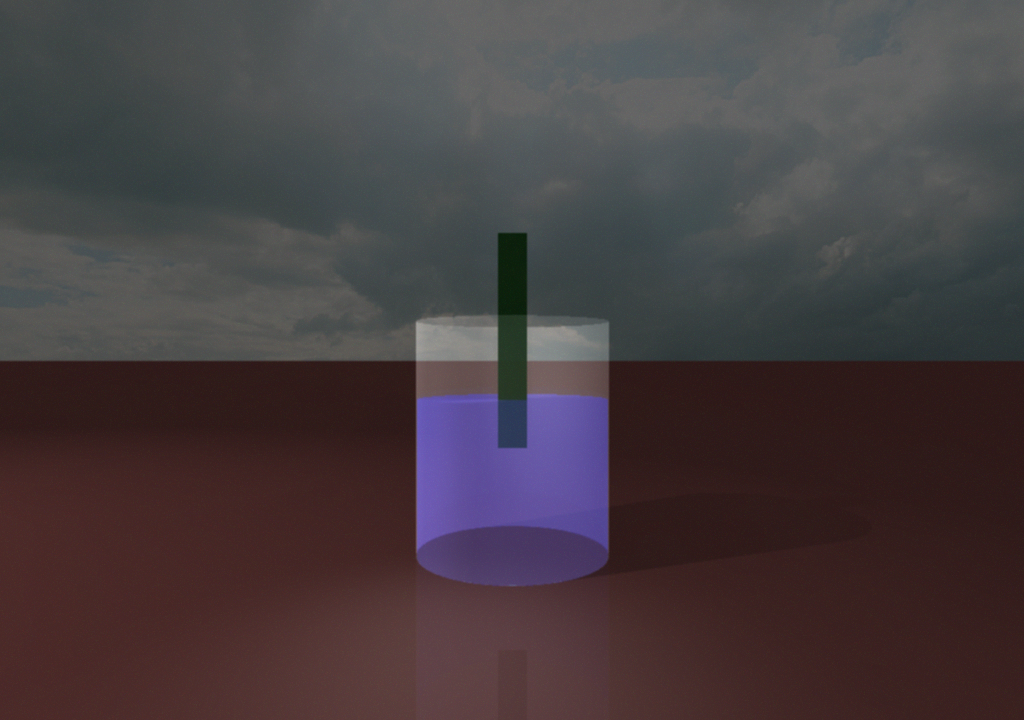
\includegraphics[scale=0.2]{img/example-1.png}
			\caption{Изображение, полученное для комбинации №1}
			\label{c1}
		\end{minipage}\hfill
		\begin{minipage}{0.45\textwidth}
			\centering
			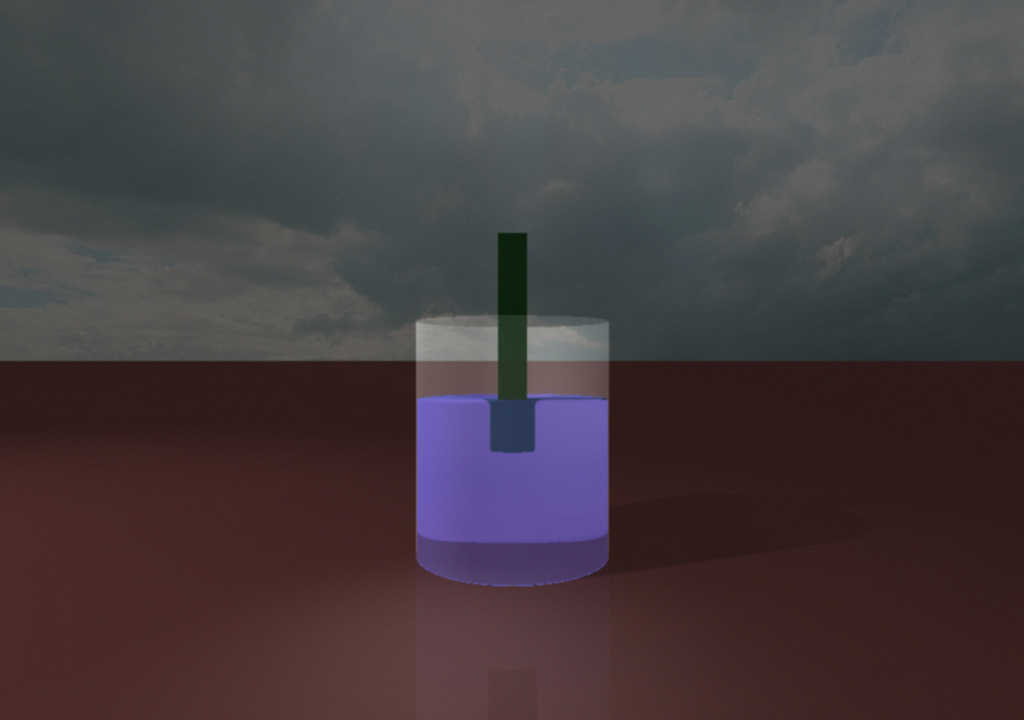
\includegraphics[scale=0.2]{img/example-2.png}
			\caption{Изображение, полученное для комбинации №2}
			\label{c2}
		\end{minipage}
	\end{center}
\end{figure}

На рисунке~\ref{c2} представлено изображение, полученное для комбинации №2 -- входных данных, где коэффициенты преломления для стекла равен 1, а для жидкости -- 1.5. Можно наблюдать более выраженное преломление света, что характерно для перехода из менее плотной среды в более плотную, как это происходит при переходе из воздуха в воду.

На рисунке~\ref{c3} представлено изображение, полученное для комбинации №3 -- входных данных, где коэффициенты преломления для стекла равен 1.3, а для жидкости -- 1. Изображение демонстрирует несколько иное поведение света, с уменьшением преломления по сравнению с предыдущим случаем, что обусловлено меньшим коэффициентом преломления для стекла.

На рисунке~\ref{c4} представлено изображение, полученное для комбинации №4 -- входных данных, где коэффициенты преломления для стекла равен 1.3, а для жидкости -- 1.5. Можно отметить комбинированный эффект увеличенного преломления как для стекла, так и для жидкости, что ведет к значительным изменениям в преломлении света при переходе через границу между двумя различными средами.

\begin{figure}[ht!]
	\begin{center}
		\begin{minipage}{0.45\textwidth}
			\centering
			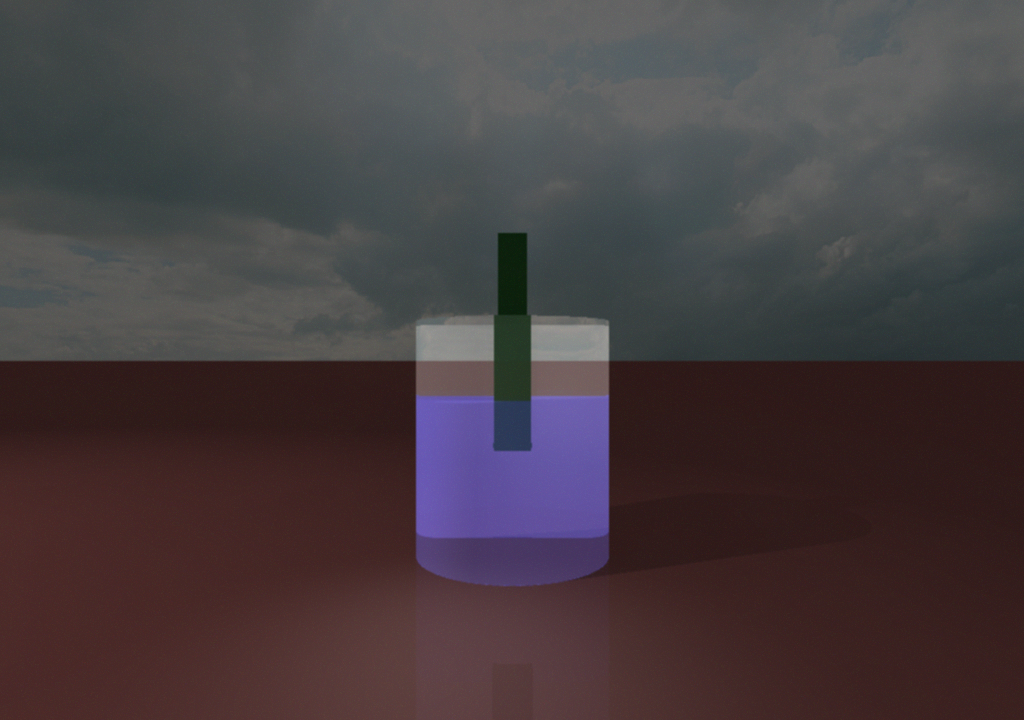
\includegraphics[scale=0.2]{img/example-3.png}
			\caption{Изображение, полученное для комбинации №3}
			\label{c3}
		\end{minipage}\hfill
		\begin{minipage}{0.45\textwidth}
			\centering
			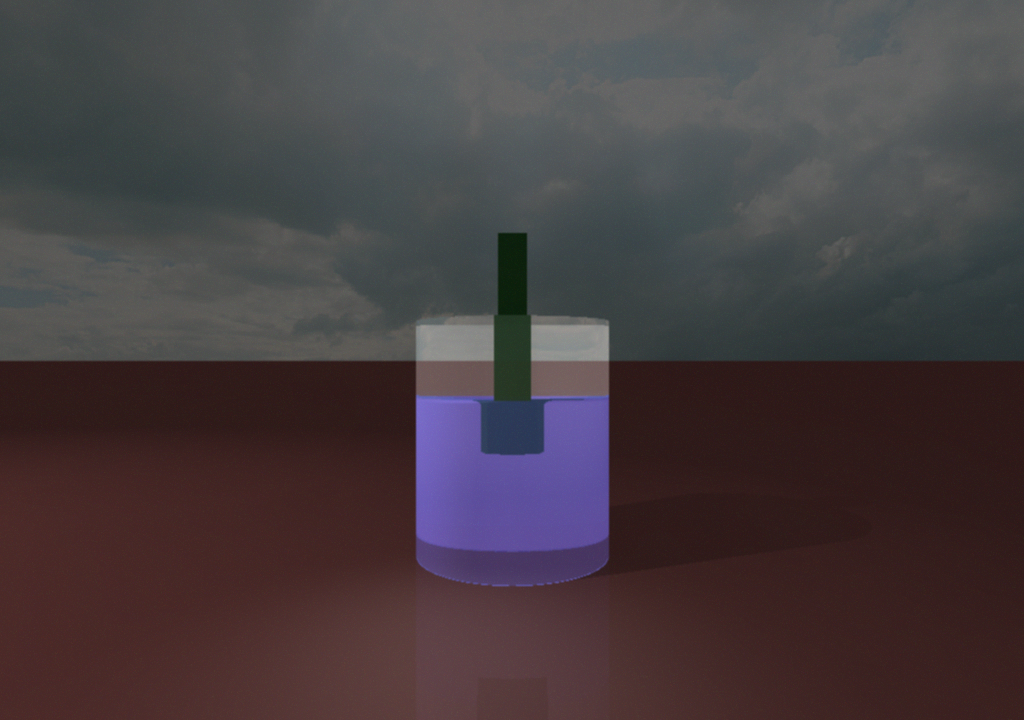
\includegraphics[scale=0.2]{img/example-4.png}
			\caption{Изображение, полученное для комбинации №4}
			\label{c4}
		\end{minipage}
	\end{center}
\end{figure}

\subsection*{Вывод}

Время построения изображения увеличивается с увеличением глубины рекурсии, что связано с увеличением сложности вычислений для каждого пикселя. Например, при глубине рекурсии 0 время выполнения составляет 2.7 секунды, а при глубине 8 -- 24.8 секунды. Эти данные подтверждают, что более высокая глубина рекурсии увеличивает время построения изображения, но также способствует более точной симуляции преломления и отражения света, улучшая реалистичность сцены.

Использование многозадачности с дополнительными потоками позволяет заметно сократить время построения изображения. Например, при использовании одного потока время выполнения составляет 5.1 секунды, а при использовании 128 потоков оно снижается до 1.08 секунды. Однако, после достижения определённого количества потоков (128 потоков) время выполнения начинает стабилизироваться, что свидетельствует о насыщении процессора и ограничениях на многозадачность. Это подтверждает, что для оптимизации времени рендеринга важна не только добавление потоков, но и балансировка их числа с учётом архитектуры процессора.

Изменение коэффициента преломления для материалов (стекла и жидкости) оказывает значительное влияние на визуализацию прозрачных объектов. В комбинации №1 (стекло и жидкость с коэффициентом преломления 1.0) изображение имеет наименьшие искажения света. В комбинациях с более высокими коэффициентами преломления, например, в комбинации №2 (где коэффициенты для стекла и жидкости составляют 1.0 и 1.5 соответственно), наблюдается более выраженное преломление света, что создаёт более реалистичное изображение при переходе через границу между двумя средами с различной плотностью. Такие изменения в коэффициенте преломления подтверждают важность точных расчётов для достижения визуальной правдоподобности при рендеринге прозрачных материалов.



